\documentclass[a4paper,11pt]{article}
\usepackage{amsmath}
\usepackage{fancyhdr}
\usepackage{graphicx}
\usepackage{url}
\usepackage{float}
\usepackage{amsmath}
\usepackage{amssymb}
\usepackage[margin=1in]{geometry}

%\setlength{\voffset}{-0.5in}
%\setlength{\headsep}{5pt}
\newcommand{\suchthat}{\;\ifnum\currentgrouptype=16 \middle\fi|\;}


%===========---------================
% Author John H Allard
% CMPE 12, Lab #1 Write-up
% October 9th, 2014
%===========---------================


\title{ CMPE 12 Lab Report \# 1 \\[7 in]}
\author{John Allard \\ TUTOR \\ MW 2:00 - 4:00pm}
\date{October 6th, 2014}

\begin{document}
\maketitle
\newpage

\section{Overview}
This lab served as an introduction to circuit design from truth tables using logic gates. All circuits were implemented using the free MultiMedia Logic (MML) program, which allows the user to drag, drop, and connect different circuit components. After the circuit is connected it can be simulated to help check for design errors. This lab consisted of 4 section, with each section varying in difficulty and length. 

\section{Part A : Using MultiMedia Logic}
\subsection{Procedure}
This section was a combined introduction to MML and DeMorgan's laws. To start we were instructed to navigate to an MML tutorial on YouTube\footnote{\url{http://www.youtube.com/watch?v=hJq2gECXYWc&noredirect=1}} and build the circuit that is shown in the tutorial. After this, we were instructed to show our understanding of MMl by implemented DeMorgans laws \(A'B' = (A+B)'\) by building a circuit for each side of the aforementioned equation and showing their equivilence both in practice and by truth table. 
\subsection{Results}
To start, we completed an extremely simple circuit on the MML software. This circuit is about as simple as one can get, it is just a binary switch connected to an LED. For the first circuit, the LED is connected directly to the switch. In this case, if the switch is high, the LED is on, if the switch is low, the LED is off. Next we simply inserted an inverter between the switch and the LED. These two circuits are shown below :  
\begin{figure}[h!]
   \centering
     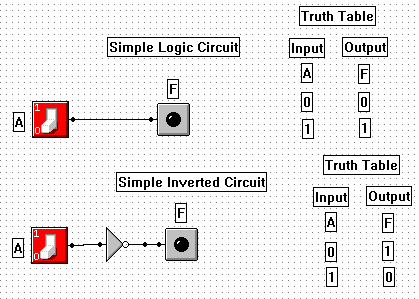
\includegraphics[width=4.4in]{PartACircuit}
   \caption{Circuit for Part A1, MML Tutorial.}
   \label{fig:map}
\end{figure} 

Our next goal was to create two new circuits which demonstrait DeMorgans law, specifically the fact that \(A'B' = (A+B)'\). This involved the use of two switch, labled $A$ and $B$. These switches will be used and the inputs for two circuits, the first one representing $A'B'$ and the second one representing $(A+B)'$. After these circuits are complete, the simulation can be run and it can be seen that the LED for each of the two circuits are in an identical state for the span of the message space, which happens to only be $ \lbrace 00, 01, 10, 11 \rbrace $ for this simple example. The first circuit, $A'B'$, is created by passing the $A$ and $B$ inputs through inverters before combining them into an AND gate. The output of the AND gate is run directly to an LED. The second circuit is made by running the $A$ and $B$ inputs directly into a NOR gate, then to an LED. The circuit and truth tables can be seen below. \\
\begin{figure}[h!]
   \centering
     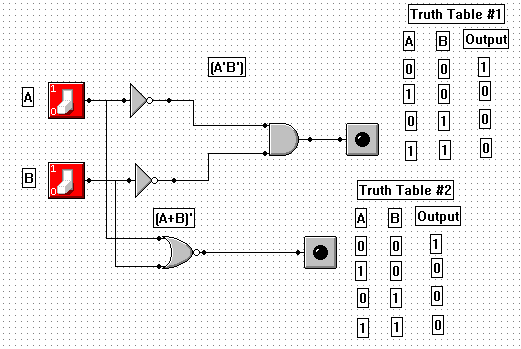
\includegraphics[width=5in]{PartADM}
   \caption{Circuits for Part A2, Showing DeMorgans Law.}
   \label{fig:map}
\end{figure}  \\

\section{Part B : Implementing Functions as Sums of Products}
\subsection{Procedure}
This part of the lab consisted of two sections. The goal of both sections was the same, implement the truth table in figure 3 (below), the differences between the two sections are the restrictions on the gates that can be used to implement the truth table.  \\ 
\begin{figure}[h!]
   \centering
     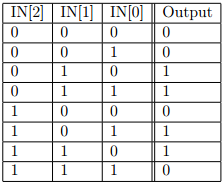
\includegraphics[width=2in]{PartBTT}
   \caption{Truth Table for Part B}
   \label{fig:map}
\end{figure} \\
In the circuits that we are building, the following names will be used for the inputs listed in figure 3 : $\text{IN[2]} \to A$, $\text{IN[1]} \to B$, $\text{IN[0]} \to C$ (reading left to right). The output of the circuit will be a single LED with a basic $1 \to \text{HIGH}$, $0 \to \text{LOW}$ relationship. Part B1 asked us to construct a circuit to represent the truth table in figure 3 using AND, OR, or Inverter gates. Part B2 asked us to reimplement the same circuit using only NAND gates. This requires translation of the AND, OR, and Inversion gates into nested layers of NAND gates. Finally, we were supposed to run the circuits in both sections side by side to ensure their equivalence. 

\subsection{Results}
Before any circuitry could be properly constructed, the truth table had to be broken down into a boolean equation using the sum of products rule. Working from left to right in the truth table in figure 3, with $\text{IN[2]} \to A$, $\text{IN[1]} \to B$, $\text{IN[0]} \to C$, we arrive at the following equation.
\[ \text{A'BC'} + \text{A'BC} + \text{AB'C} + \text{ABC'} \]
Also this equation can be simplified significantly, we were instructed to not simplify it before designing our circuits. 
\begin{itemize} 
\item \textbf{Part B1 - AND, OR, \& NOT Gates}
\item \textbf{Part B2 - NAND Gates}
\item
\end{itemize}

\section{Part C : Logic Minimization}
\subsection{Procedure}
\subsection{Results}

\section{Part D : Guessing Game}
\subsection{Procedure}
\subsection{Results}
\section{Results}


\end{document}